\documentclass[12pt, a4paper]{scrartcl}
\usepackage[utf8]{inputenc}     %% adapte le style article aux conventions francophones
\usepackage[english]{babel}
%\frenchbsetup{StandardLists=true} 
\usepackage[T1]{fontenc}          %% permet d'utiliser les caractres accentus
\usepackage{graphicx}      %% \usepackage[dvips]{graphicx}      %% permet d'importer des graphiques au format .EPS (postscript)
\usepackage{makeidx}              %% permet de gnérer un index automatiquement
\usepackage{authblk}
\usepackage{hyperref}
\usepackage{enumitem} 
\usepackage{pdfpages}
\usepackage{wasysym}
\usepackage{listings}
\usepackage{dirtree}
\usepackage{array}
%%% HEAD
\begin{document}

\author{Dominique Benielli}
\affil{\itshape Labex Archim\`ede \upshape}
\title{User Guide for OPTMISME}
\subtitle{OPTIMIsation Stochastique en imagerie MultispectralE,\\ Image-J plugin}
%%\subtitle{plugin pour ImageJ sur Imag’In OPTIMIsation Stochastics en imagerie MultispectralE }

\maketitle
\begin{center}

\includegraphics[scale=0.2]{images/logo_labex.jpeg}
\end{center}
\tableofcontents                  %% la table des matieres		

%% \newpage

%%% SECTION
\section{Introduction}
\subsection{Historical development}
The scientific project was at first a french project for young researchers financed by the Gdr ISIS in 2013.
It then continued and extended with the financial support of CNRS within the project Imag'In in 2015-2016 under the name OPTIMISME for \emph{OPTIMIsation Stochastique en imagerie MultispectralE} i.e. Stochatic Optimization in Multispectral Imagery.

This project focuses on the restoration of two-photon microscopy data. It is composed of two parts: a theoretical approach and its application to two-photon microscopy data.

In the theoretical part, proximal algorithms have been developed, one of them is based on a Majorization-Minimization procedure.
In the applicative part, the developed algorithms were used to  restore two-photon  microscopy images. 
Furthermore this approach included an analysis of the noise and the non-stationarity of the PSF.

\subsection{Abstract}
Modern approaches of inverse problems resolution in the field of multi- or hyper-spectral imaging are based on variational formulations.
The goal of this study is to provide a generalization of parallel methods using recent 
advances of stochastic optimization, for the treatment of massive big data.
The  algorithms provided solve the multispectral deconvolution problem in two-photon microscopy.

\subsection{Scientific issues}
The in-vivo observation of a mouse brain by a two-photon microscope leads to direct images at cellular scales, which are degraded by blur and noise and need restoration.
This problem yields an inverse problem that was targeted by the OPTIMISME project.
The issue of obtaining the PSF of the two-photon microscope was solved by observing fluorescent micro beads (of diameter 0.5 $\mu$m) at different depths. The PSF varies with the depth ($z$ coordinate).
The OPTIMISME-ImageJ plugin implements the Majorization-Minimization proximal algorithm described in~\cite{chouzenoux:hal-01278102} to restore an image that has been blurred by a known PSF.

\subsection{ImageJ}
ImageJ is an image processing software dedicated to multidimensional scientific images.
ImageJ can be easily extended adding plugins and scripts.
ImageJ web site:
\begin{itemize}
\item 
\href {http://imagej.net/Welcome}{imageJ homepage}
\end{itemize} 


\section{Plugin OPTIMISME}

ImageJ gives the possibility to user to develop and install one's own plugin. The following page explain how to install an ImageJ plugin :
\begin{itemize}
\item 
\href  {http://imagejdocu.tudor.lu/doku.php?id=howto:plugins:how\_to_install\_a\_plugin} {imageJ Plugin Install}
\end{itemize} 


%\subsection{Public Distribution}
%For version 1.0 a recording of the plugin by the mechanism of ImageJ plugin registration is %needed. We recommended a private site repository lighter than the imageJ git repository.
% \begin{itemize}
% \item \href {http://imagej.net/How\_to\_set\_up_and\_populate\_an\_update\_site}{update%\_imageJ} 
% \end{itemize} 
 
%\begin{lstlisting}[language=bash]
%$ git clone git@git.math.cnrs.fr:forge/optimisme
%$ cd optimisme/Toolbox_optimism
%\end{lstlisting}

\subsection{Libraries}
Libraries used for the OPTIMISME algorithm are:
\begin{itemize}
 \item \textit{edu.emory.mathcs.jtransforms }
 For 3D and 2D FFT and IFFT.  On license BSD clause 2. Non contaminant license.
 \item  \textit{org.ejml} a part of ejml library for matrix calculus and pseudoInvers function. On Apache license Non contaminant license.
 \item \textit{org.apache.commons.math3} a part of apache common library for tricubic interpolation. on Apache license Non contaminant license.
\end{itemize}

\subsection{System requirements}
The OPTIMISME plugin requires version 1.48 or higher of ImageJ (or Fiji) and java 8 or higher. (To check your installation click on \emph{Help>About ImageJ..}, the java version must be 1.8.0 or higher).

\subsection{Installation}
The plugin OPTIMISME is available under the following formats.

\subsubsection{Private Distribution, .class}
 To install it, 
  \begin{itemize}
\item Add the directory OPTIMISME in the plugin directory of ImageJ (or Fiji) (with all the *class files). Then 
 start ImageJ (or Fiji).
 
\item If the plugin item "OPTIMISME" does not appear in the menu : Go to Help>Refresh Menus or (better) restart ImageJ (or Fiji). 
\end{itemize} 

% The renaming of the java file comes from incompatibility  between imageJ and  fiji compilation.
\subsection{Public Distribution}
If you are using Fiji, it is possible to install the plugin through the public distribution using the install plugin menu (\emph{Plugins>Install PlugIn..}).

\subsubsection{Private Distribution, .java}
For earlier versions of ImageJ or Java, it may be necessary to compile the plugin. The java files are available in the OPTIMISME folder. To compile them, 
   \begin{itemize}
   \item Add the directory OPTIMISME in the plugin directory of ImageJ.
   \item Rename the file \textit{optimisme.txt} as  \textit{optimisme\_.java}.
   \item Start ImageJ. 
   \item Click on Plugins > Compile and Run.
   \item Select the  file \textit{optimisme\_.java}.
   \item If the plugin item "OPTIMISME" does not appear in the menu : Go to Help>Refresh Menus or (better) restart ImageJ. 
  \end{itemize} 
  
% \subsection{Private Distribution, .jar}
%  
% Copy the OPTIMISME.jar file to the ImageJ/Plugins folder plugin/jars
% Go to Help>Refresh Menus or (better) restart ImageJ. 
%
\subsection{Launch}
The Plugin is accessible through the ``Plugins'' menu of ImageJ.
The OPTIMISME plugin  assumes that at least two images are opened: the image to restored and the PSF. 
Note that the present version is established with one single PSF.  

Launch the OPTIMISME Plugin as follows:

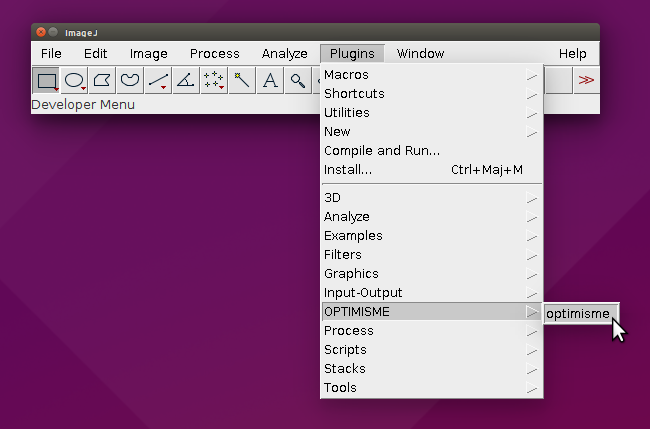
\includegraphics[scale=0.3]{images/lancerOptimisme.png}

In the first window of the plugin OPTIMISME, the user specifies the input image,  the channel that needs restoration, and the PSF image. Others parameters of the algorithm described hereafter, may also be specified (see~\cite{chouzenoux:hal-01278102} for more details).

\subsubsection{Input parameters}
In the window of OPTIMISME Plugin, the Input parameters have default values, that can be modified by the user.
\begin{center}
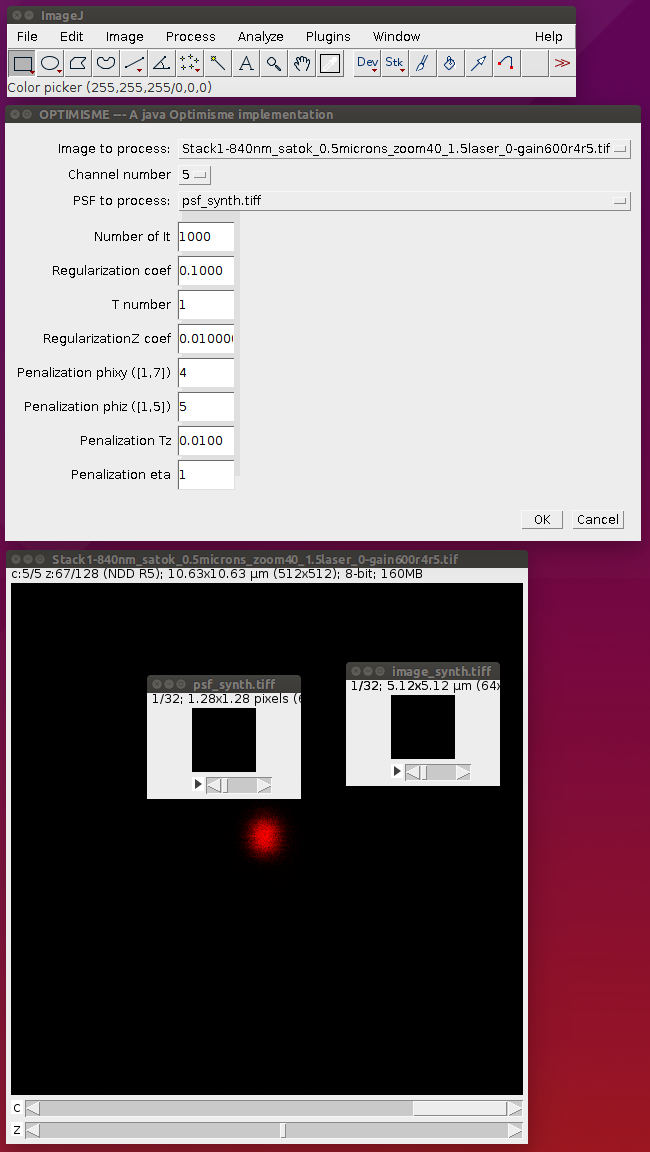
\includegraphics[scale=0.3]{images/plugginI.png}
\end{center}
 \begin{itemize}
 \item  NbIt: number of iteration of the algorithm that are performed.
 \item  regul: regularization coefficient for $XY$ coordinate (space)
 \item  T:  smoothing parameter for the $XY$ regularization term
 \item  regulZ: regularization coefficient for the $Z$ coordinate (depth)
 \item  phixy: choice of the $XY$ regularization function
 \item  phiz: choice of the $Z$ regularization function
 \item  TZ: smoothing parameter for the $Z$ regularization term
 \item  eta: regularization parameter to force the solution to be positive
 \item  Channel number: in case the input image contains several channels, the user can select the channel to restore.
  \end{itemize}


\subsection{Input Files}
Before you launch OPTIMISME, you have to open two images corresponding to 1) the image to be processed and 2) the PSF to be used.
OPTIMISME needs as input file two images (image and PSF). ImageJ accepts different formats (tiff format, lsm directly issued from microscope...).
\begin{itemize}

 \item File>Open open at least two files one for Image and one for the PSF.
OPTIMISME assumes 3D files, images with a depth dimension.

 \end{itemize}




\subsection{Computations}
The algorithm first compares the resolutions of the image and the PSF: if resolutions are different the  PSF is re-sampled to the resolution of the image; at the end of this first stage the re-sampled PSF is plotted (it may then be stored by the user for a later use).
The plugin then proceeds with the actual restoration algorithm (see~\cite{chouzenoux:hal-01278102} for more details), and finishes by plotting of the processed image.

\subsection{Results}

The OPTIMISME plugin outputs at least one image
\begin{itemize}

\item At the end of the computations an image is opened: it is the deconvolved image, the user can save it using the   menu.
\item When the input images (image and PSF) do not have the same resolution, the algorithm first re-samples the PSF; then, at the end of this first stage, the program displays the re-sampled PSF with the same resolution as the input image. The user can save it for further runs of the program and use it for all the images having the same resolution  using the \emph{File>Save as} menu.
\end{itemize}
\subsubsection{others Output}
At the end of the calculation a text OPTIMISME software open a text window that summarizes the different parameter used for the previons calculation, this file can be save as txt file with th menu \emph{File>Save as}

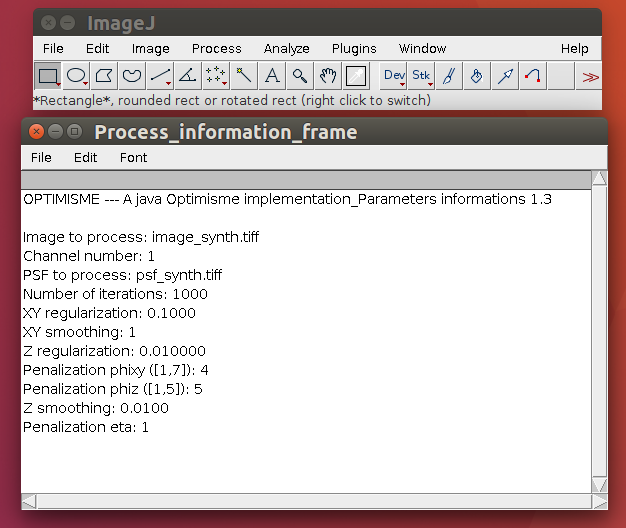
\includegraphics[scale=0.3]{images/txtWindow.png}
\section{Package OPTIMISME}

\subsection{The java class}
The java class of algorithm Majorization/Minimization
in ImageJ plugin, and other dependencies
\dirtree{%
.1 /ImageJ/plugins/OPTIMISME/.
.2 org.jar.
.2 fftj.jar.
.2 doc/.
.3 \textit{index.html}.
.3 \textit{...}.
.2 \textit{optimisme\_.java}.
.2 data.
.3 \textit{image\_synth.tiff}.
.3 \textit{psf\_synth.tiff}.
.3 \textit{psf\_synth\_subsampled.tiff}.
.2 optimisme.
.3 \textit{MM.java}.
.3 \textit{PSFPreparator.java}.
.3 \textit{MMCal.java}.
.3 test.
.4 \textit{AllTests.java}.
.4 \textit{MMCalTest.java}.
.4 \textit{MMTest.m}.
.4 \textit{PSFPreparatorTest.m}.
}
\subsection{Test Coverage}
Tests files are in the test folder. The coverage by Emma leads to :

\begin{center}
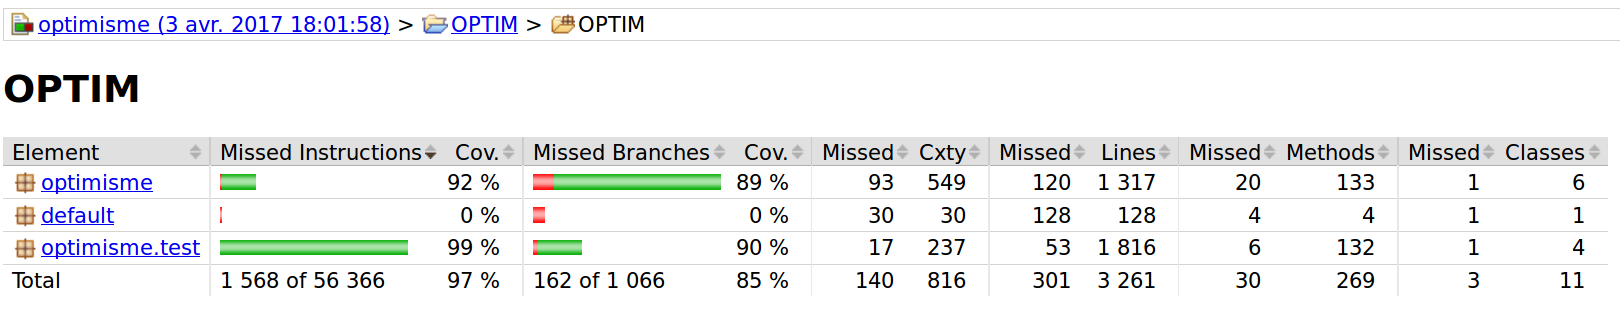
\includegraphics[scale=0.28]{images/coverage1.png}
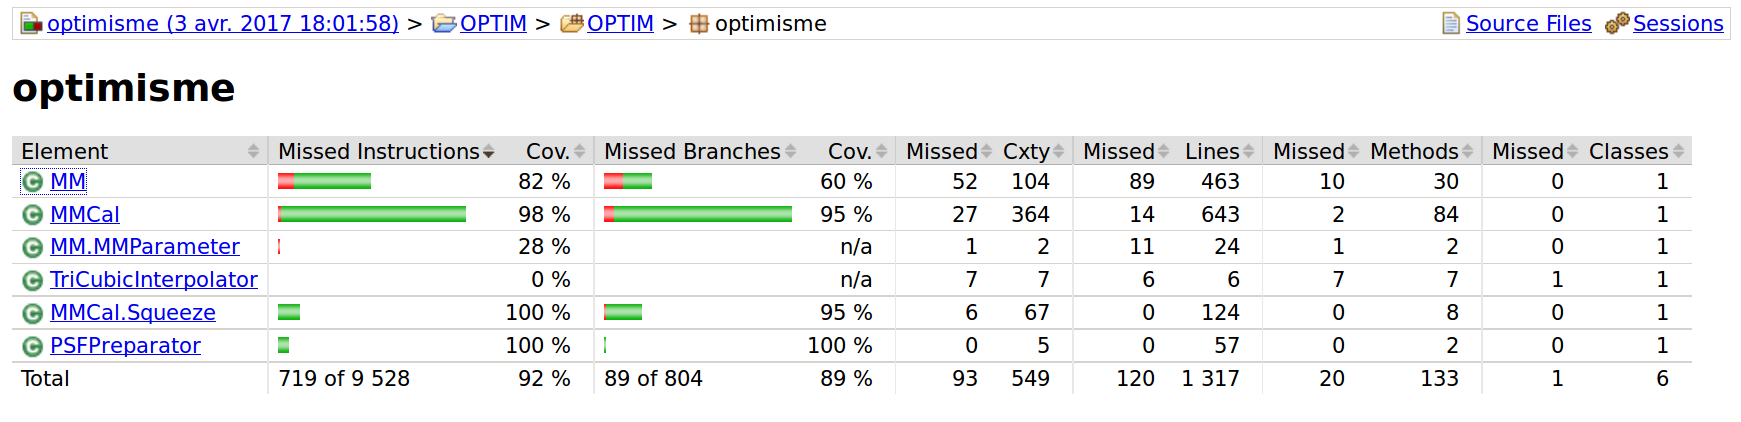
\includegraphics[scale=0.28]{images/coverage.png}
\end{center}


\subsection{Tests}
\begin{tabular}{lllll}
   source files   &       file size    &  \%CPU & \%MEM & \%TIME \\
   stark1\_840 *2 &  342 (512*512*261) &  100   & 61    & 763 -stop \\
   stark1\_450 *2 & 225 (512*512*172)  &  100   & 61    & 763 -stop\\
   stark1\_840 * psf\_synth & 167 (512*512*128) &  100  & 7.4  & 22:20? \\
   stark1\_840 * psf\_synth & 167 (512*512*128  & 324 & 81  & 3:00 \\
\end{tabular}


\begin{thebibliography}{2}

\bibitem{chouzenoux:hal-01278102}
E.~Chouzenoux, L.~Lamasse, S.~Anthoine, C.~Chaux, A.~Jaouen, I.~Vanzetta, and
  F.~Debarbieux.
\newblock {Approche variationnelle pour la d{\'e}convolution rapide de
  donn{\'e}es 3D en microscopie biphotonique}.
\newblock In {\em {Actes du 25e colloque GRETSI}}, Lyon, France, September
  2015.
\end{thebibliography}

\end{document}
